\setcounter{chapter}{2}
\setcounter{section}{0}
\part{FUNDAMENTACIÓN TEÓRICA DE LA INVESTIGACIÓN}

\section*{FUNDAMENTACIÓN TEÓRICA}
En este capítulo, se expondrán los trabajos relacionados con el presentado en este documento que se han identificado en la literatura, y que demuestran que el trabajo propuesto en este documento, aporta algo. Además, se contextualiza el trabajo y define los términos novedosos y de poco dominio para los investigadores y para la comunidad.

\section{Marco conceptual}

En esta sección, se detalla los modelos teóricos, conceptos, argumentos o definiciones que se han desarrollado o investigado en relación con el tema en particular.


\subsection{Lenguajes de marcado}	

A continuación, se describen una serie de formatos de texto utilizados para el intercambio de datos entre varias aplicaciones.

\subsubsection{JSON}

Javascript Object Notation (JSON) es un formato ligero de intercambio de datos. Consisten en asociación de nombres y valores. A pesar de ser independiente del lenguaje de programación, es admitido en una gran cantidad de lenguajes de programación. Se basa en un subconjunto del Estándar de lenguaje de programación JavaScript \cite{JSON}.

\begin{figure}[h!]
	\caption{Estructura json.}
	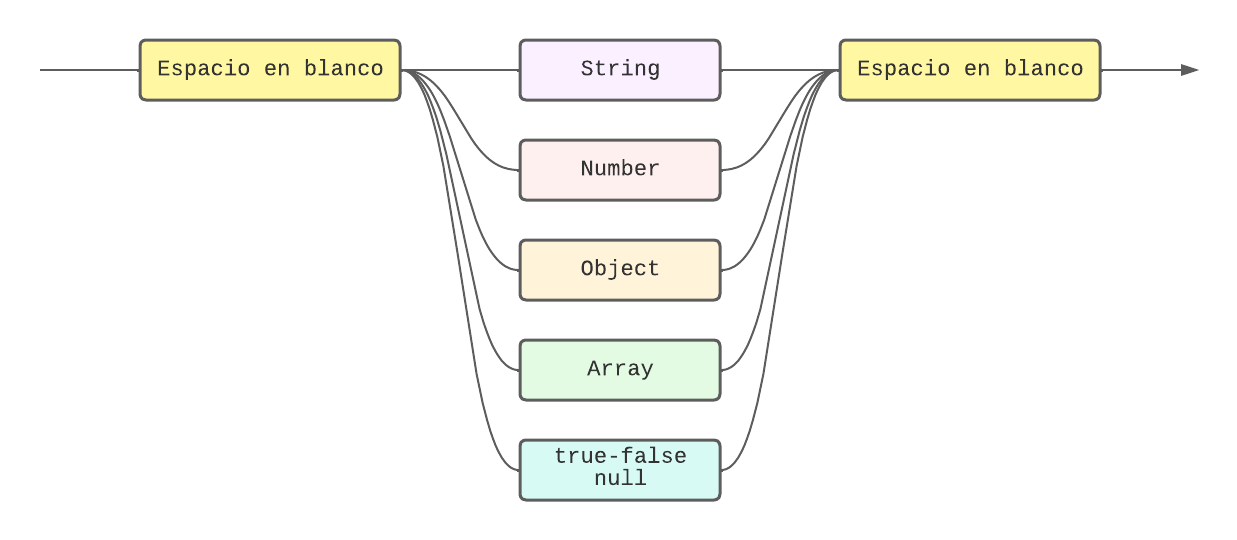
\includegraphics[width=12cm]{img/json.png}
	\label{fig:json}
	\textbf{\\ FUENTE: PROPIA \\ ELABORADO: DÚVAL CARVAJAL SUÁREZ} 
\end{figure}

\subsubsection{XML}

Es un lenguaje de marcado similar a HTML. Significa Extensible Markup Language y pertenece a la especificación W3C como lenguaje de marcado de propósito general. Esto significa que, a diferencia de otros lenguajes de marcado, XML no está predefinido, por lo que debe definir su propio marcado. El objetivo principal del lenguaje es compartir datos entre diferentes sistemas, como Internet \cite{XML-based}.

\begin{figure}[h!]
	\caption{Estructura xml.}
	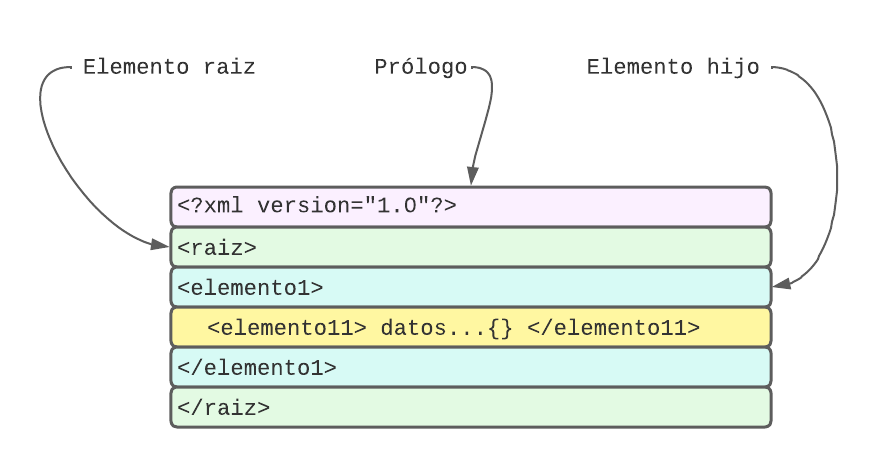
\includegraphics[width=12cm]{img/xml.png}
	\label{fig:xml}
	\textbf{\\ FUENTE: PROPIA \\ ELABORADO: DÚVAL CARVAJAL SUÁREZ}
\end{figure}

\subsection{Compiladores}
Están diseñados para traducir un fragmento de código escrito en un de lenguaje de programación a lenguaje de máquina que es, el que puede entender la computadora. El compilador analiza el código fuente en busca de errores antes de la traducción. Si se detecta un error, el compilador
notificar al autor del código para que pueda arreglarlo. Además, los compiladores modernos o entornos de desarrollo (IDE), puede sugerir soluciones para algunos tipos de errores usando métodos de corrección de errores \cite{CoEdit}.

\subsection{Modelamiento de software}
Representan una serie de requisitos basados en la construcción de elementos visuales para definir estructuras y comportamientos que tendrá el software. UML (Lenguaje Unificado de Modelado) a través del mecanismo de perfilado, se han basado históricamente en notaciones gráficas. UML mediante el mecanismo de perfiles, maximiza la comprensión humana y facilita la comunicación entre las partes interesadas como son el cliente y desarrollador \cite{Blended}. 

También existen lenguajes de modelado personalizados para distintas áreas, como por ejemplo en \cite{Multi-level} proponen un lenguaje de modelado conceptual multinivel al denominan ML2 (Lenguaje de Modelado Multinivel). El lenguaje está orientado al modelado conceptual multinivel (de dominio) y pretende cubrir un amplio conjunto de dominios multiniveles. En el diseño de ML2 sigue un enfoque basado en principios, definiendo su sintaxis abstracta para reflejar una teoría formal para el modelado multinivel que se fue desarrollado previamente.

\subsection{Metamodelado}

Existen varias formas de realizar el metamodelado de un software. En \cite{Mohamed} mencionan el \textit{Software Pattern MetaModel} (SoPaMM) o en su traducción al español Metamodelo del patrón de software. El objetivo principal de este proceso es la especificación de patrones de requisitos funcionales (FRP) vinculados a patrones de pruebas de aceptación (ATP). En la figura \ref{fig:metamodelo} se observa los componentes más importantes de un FRP relacionado con un ATP.

Basada en metodología ágil BDD, FRP es una estructura inspirada en la descripción de las historias de usuario. A continuación, se detalla la estructura de un FRP \cite{Mohamed}:

\begin{itemize}
	\item \textbf{As: }Describir la parte que se beneficia de la característica.
	\item \textbf{I\_can: }La característica en sí.
	\item \textbf{So\_that:} El valor agregado de la característica.
	\item \textbf{Given:} Describe, en una o más cláusulas, el contexto inicial del escenario.
	\item \textbf{When:} Describe los eventos que desencadenan un escenario.
	\item \textbf{Then:} Describe, en una o más cláusulas, los resultados esperados del escenario.
\end{itemize}

\begin{figure}[h!]
	\caption{La estructura y los contenidos de un FRP asociado a un ATP.}
	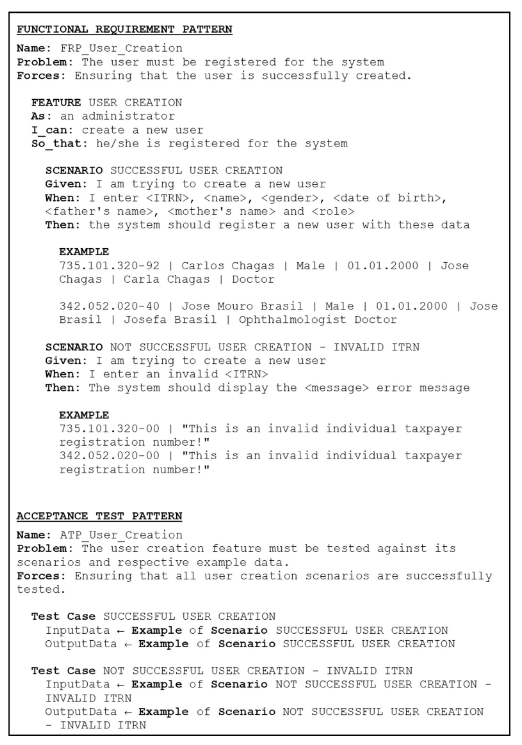
\includegraphics[width=15cm]{img/metamodelo.png}
	\label{fig:metamodelo}
	\textbf{\\ FUENTE: \cite{Mohamed} \\ ELABORADO: DÚVAL CARVAJAL SUÁREZ}
\end{figure}

Como se observa en la figura \ref{fig:metamodelo_sopamm} FRP\_User\_Creation describe una parte de la función para crear usuarios. Se puede visualizar que el usuario administrador es el actor beneficiado de esta función para que se logre registrar un nuevo usuario al sistema. El intento de crear un usuario conlleva a dos posibles escenarios: uno exitoso y otro no exitoso, pero ambos vinculados a una misma precondición.  Sin embargo, dependiendo de la validez de los usuarios la ejecución puede ser distinta. Del mismo modo por cada escenario se representará un resultado diferente, es decir se visualizarán mensajes diferentes al momento de registrar un usuario o mensajes de error \cite{Mohamed}.

Finalmente, el ejemplo mostrado permite definir y vincular varios datos cada escenario. En cada escenario se consta con dos instancias de datos, de manera que uno de los escenarios registrado un nuevo usuario con éxito, mientras que el otro no lo hace debido a que los datos de entrada no son válidos, como es el número de identificación del usuario. Esta representación define el enfoque de patrones de requisitos funcionales basado en la ejecución de los posibles escenarios. En la figura \ref{fig:metamodelo_sopamm} se observa el metamodelo de SoPaMM \cite{Mohamed}.

\begin{figure}[h!]
	\caption{El metamodelo SoPaMM.}
	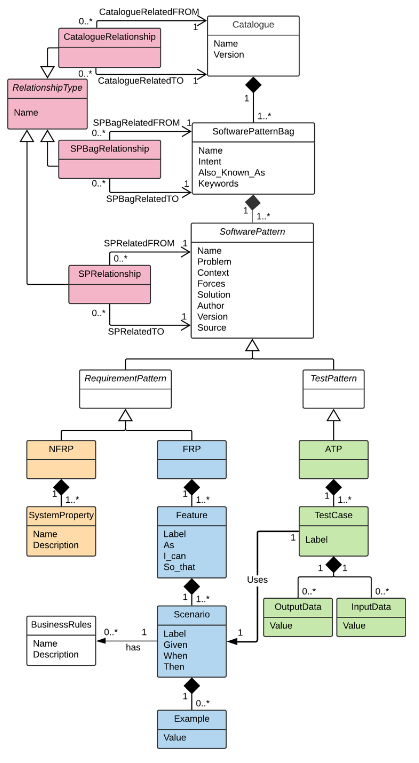
\includegraphics[width=10cm]{img/metamodelosopamm.png}
	\label{fig:metamodelo_sopamm}
	\textbf{\\ FUENTE: \cite{Mohamed} \\ ELABORADO: DÚVAL CARVAJAL SUÁREZ}
\end{figure}


\subsection{Desarrollo ágil de software}

El desarrollo ágil de software hace referencia a los principios del manifiesto ágil que son aplicadas por varias metodologías de desarrollo. Las metodologías de desarrollo ágil comparten varias características como: la entrega frecuente de software de trabajo (desarrollo iterativo), la velocidad constante y la comunicación abierta \cite{Whiting2022}. En el desarrollo ágil los métodos que se emplean pueden ser de bajo costo, es decir que cualquier modificación que se realice en alguna etapa de desarrollo el cliente podrá observar los resultados deseados referente al costo que ha pagado \cite{Shafiq2018}. 

Además, de ser una buena alternativa para mejorar el desarrollo de software, el desarrollo ágil es muy productivo por que brecha de comunicación entre los clientes y los desarrolladores de software. Conforme avance el tiempo, difícilmente pueden surgir motivos para generar retrasos. Lo beneficioso de aplicar este proceso es que los cambios pueden ser acoplados continuamente de acuerdo a las necesidades del cliente. A continuación, se mencionarán varias metodologías ágiles que se utilizan en el desarrollo de software \cite{Shafiq2018}:

\begin{itemize}
	\item \textbf{La programación extrema (XP):} Esta es una metodología centrada específicamente en obtener un software de calidad. Para cumplir con ese objetivo, se debe considerar en primer lugar una buena comunicación verbal entre todos los integrantes del proyecto. Además, no existen reglas que obliguen a llevar una documentación rigurosa, con el fin de aumentar la eficiencia de desarrollo del software.
	
	\item \textbf{Dynamic Systems Development Method (DSDM): }En DSDM o en su traducción al español Sistemas dinámicos Método de desarrollo la documentación es totalmente necesaria, debe ser magra y oportuna describiendo paso a paso todo el proceso que se realizó. Esto significa que el modelo y el prototipo deberán representar una visión general sobre lo que va hacer el sistema. Además, se deberán documentar los diagramas de modelado, estructuras físicas de datos y decisiones de diseño.
	
	\item \textbf{Scrum: } Se centra netamente en la versatilidad rentabilidad y adaptabilidad. Le permite al desarrollador tomar la decisión para elegir la técnica de ejecución del módulo que este encargado. La administración de Scrum permite reconocer las carencias u obstáculos que se presentaran a lo largo del proyecto. Los equipos de Scrum tienen la libertad de elegir y reconocer los enfoques para realizar su trabajo, es decir que cada integrante del grupo cuanta con las habilidades necesarias para cumplir su trabajo sin necesidad de recurrir a pedir ayuda fuera del grupo.
\end{itemize}

\section{Marco referencial}

El diagrama de clases sin duda es el artefacto más importante para modelar un sistema y el punto de partida para otros diagramas \cite{Tan2010}. La problemática de la obtención de diagramas de clases a partir de los casos de uso detallados no ha sido tratada a profundidad. Por lo tanto, los investigadores se encuentran en un campo fértil de investigación.

Las soluciones que se han propuesto y que se han recuperado en este trabajo, utilizan el procesamiento del lenguaje natural (NLP por sus siglas en inglés \textit{Natural Language Process}). Entre las soluciones encontradas podemos mencionar el trabajo de Chen y Zeng \cite{Chen2010}, en el cual presentan una aproximación sobre la obtención del diagrama de casos de uso y el diagrama de clases UML a partir de los requisitos del producto expresados en lenguaje natural. Sin embargo, en este trabajo intentan analizar el texto para determinar el conjunto de palabras significativas que pueden representar los elementos de los diagramas, por ejemplo, para una clase un sustantivo, para un método un verbo nominal para los métodos, la conexión entre dos objetos (clases) expresarían una relación. El trabajo de Chen \& Zeng \cite{Chen2010} tiene buenos resultados con pocos y bien establecidos requisitos de software, que pueden animar a los investigadores a seguir mejorando esa herramienta, cómo por ejemplo, identificar los diferentes tipos de relaciones entre clases, y su representación en el diagrama UML.

El trabajo presentado por Dawood Omer \& Eltyeb \cite{Dawood2022} es otra de las soluciones propuestas. En \cite{Dawood2022} proponen un modelo de razonamiento que basado en casos puede facilitar el proceso de generación de diagramas de clases UML a partir de requisitos textuales. Para ello utilizan técnicas de minería de texto. Por lo tanto, el trabajo es bastante abrumador: primero se deben tener una base de casos para entrenar el modelo, luego se debe entrenar el modelo. Además, aunque las diferencias sean muy pequeñas, los resultados (diagrama de clases UML) puede variar.

En la misma línea de la aplicación de procesamiento del lenguaje natural para la obtención del diagrama de clases a partir de la descripción textual de los requisitos, podemos citar el trabajo de Abdelkareem M. Alashqar \cite{Alashqar2021}, en el que, para lograr este objetivo proponen un algoritmo y una herramienta. El algoritmo consiste básicamente en la separación de la oración en cada palabra que la conforman para luego aplicar un análisis morfológico a cada palabra, según el tipo de palabra (sustantivo, verbos en diferentes voces o tiempos, etc.) determinar los diferentes elementos de los diagramas. En este caso, la herramienta que implementan para aplicar el algoritmo muestra las oraciones que han sido mal escritas. Alshgar en su trabajo \cite{Alashqar2021} especifica que, para el algoritmo funcione correctamente, los requisitos textuales deben estar escritos con ciertas restricciones, cómo por ejemplo: cada oración debe estar escrita en una línea (separadas con una nueva línea), y que cada oración represente una acción a realizar con el software, entre otras restricciones. 

De los trabajos que se revisado hay que recalcar que \cite{Alashqar2021} y \cite{Shweta2020} se preocupan por el análisis de oraciones (acciones) pasivas negativas. Sin embargo, todos los trabajos que utilizan NLP están limitados al idioma en el que están escritos los requisitos, y al uso correcto de la gramática y todos consideran restricciones en la escritura. Por lo que se presenta a Armadillo como una librería que ayuda que SymLen sea un lenguaje a utilizar para la escritura de los casos de uso detallados sin importar el idioma, y sin ninguna restricción. Con Armadillo la eficiencia de los diagramas de clases y la generación de código de software que satisface los requisitos del usuario, depende estrictamente del uso correcto de SymLen, y/o de la corrección de los posibles errores de su uso que Armadillo muestre al analista.



